\section*{Contents of the dissertation}

% Is there no way to pull the chapter numbers from the main document? 
\textbf{The first chapter} introduces the necessary definitions and ideas of quantum computation. Section 1.1 introduces quantum states, unitary, Hermitian, and Pauli operators. Section 1.2 presents the key concepts of the quantum model of computation: quantum circuits, quantum gates, and measurements. Section 1.3 describes the formalism necessary to describe quantum states and their evolution in the presence of noise. Section 1.4 briefly presents the language of tensor networks. Finally, Section 1.5 reviews the complexity-theoretic aspects of quantum computing. We present the common complexity classes $\mathbf{P}, \mathbf{BPP}, \mathbf{NP}$ and their quantum counterparts $\mathbf{BQP}, \mathbf{QMA}$.

\textbf{The second chapter} introduces the idea of variational quantum algorithms and reviews state-of-the-art techniques in the field. The key observation underpinning the variational methods is called the Rayleigh-Ritz variational principle (Section~2.1). Let $H$ be a Hermitian operator on a finite-dimensional Hilbert space $\mc{H}$, and let $ \ket{\psi(\theta)} \in \mc{H}$ be an arbitrary family of states parametrized by a vector of parameters $\theta \in \mathbb{R}^k$ for some $k$ (such family of states will henceforth be called an \textit{ansatz}). The ground state energy $E_{gs}$ (i.e.~the lowest eigenvalue of $H$) satisfies the following inequality:
\begin{equation}
    \label{eq:variational_principle}
    E(\theta) = \frac{\bra{\psi(\theta)} H \ket{\psi(\theta)}}
         {\braket{\psi(\theta)}{\psi(\theta)}} \geq E_{gs}.
\end{equation}
This means that if we pick $\theta$ so that $E(\theta)$ is minimal, we can find a state that is the best approximation of the ground state in the sense of energy error. The remainder of Section 2.1 works through a simple example of this principle applied to a spin model.

Section 2.2 describes the variational quantum eigensolver (VQE) algorithm. Given a Hamiltonian $H \in \operatorname{Herm} (2^n)$ and an ansatz $\ket{\psi(\theta)}$ that is a differentiable function of $\theta \in \mathbb{R}^k$ for some $k$, this algorithm finds an approximate value of the ground state energy $E_{gs}$. A simple description of VQE is the following loop:
\begin{enumerate}
    \item Estimate $E(\theta) = \bra{\psi(\theta)} H \ket{\psi(\theta)}$. 
    \item Use a classical optimization routine to find the next value of $\theta$. If the new value of $\theta$ is different from the old value by a threshold smaller than $\epsilon$, stop.
\end{enumerate}
The value of $E(\theta)$ in the last iteration is the output of the algorithm. 

There are two important details to point out:

\begin{enumerate}
    \item In step 1, the estimate of $E(\theta)$ is sometimes replaced by the estimate of $\nabla E$, depending on the optimization routine in step 2.
    \item The value $\bra{\psi(\theta)} H \ket{\psi(\theta)}$ is not easy to evaluate for any Hamiltonian. To be able to do that, we need to put additional restrictions on $H$. More precisely, we need $H$ to consist of a polynomial number of operators $h_i$ such that every expectation $\bra{\psi(\theta)} h_i \ket{\psi(\theta)}$ can be measured in polynomial time. An example of a Hamiltonian the conforms to this restriction is a Hamiltonian that consists of a polynomial number of Pauli strings. Alternatively, the Hamiltonian can consist of a polynomial number of projectors on product states.
\end{enumerate}
The rest of Section 2.2 reviews the optimization methods, the methods of estimating the gradients on quantum hardware, and the choice of the ansatz states.

Section 2.3 describes the sequence of actions necessary to apply VQE to the problem of electronic structure of a molecule. Section 2.4 discusses other applications of VQE. Section 2.5 reviews advanced variants of the algorithm. Section 2.6 reviews other variational quantum algorithms.

\textbf{The third chapter} presents our results on VQE for physical models. The chapter begins with a review of existing literature on the subject (Section 3.1). Section 3.2 presents the results of using VQE on spin models. The first model of interest is the transverse field Ising (TFI) model:

\begin{equation}\label{eq:tfim}
    H_\mathrm{TFIM}=J\sum\limits_{i=1}^n Z_i Z_{i+1} + h\sum\limits_{i=1}^n X_i, \; J>0, \; h>0.
\end{equation}

The numerical solutions for the ground state problem are found using different ans\"atze. The dependence of energy error on the ansatz choice and the value of $J$ is shown in Figure \ref{fig:dE_ising}. The curves were obtained using the variant of the algorithm called adiabatically-assisted VQE (AAVQE)~\cite{garcia-saez_addressing_2018}. This variant is applicable to situations when one needs to find solutions to a series of similar problems. Its idea is to initialize the optimization for the next problem with the solution of the previous problem.

\begin{figure}
    \centering
    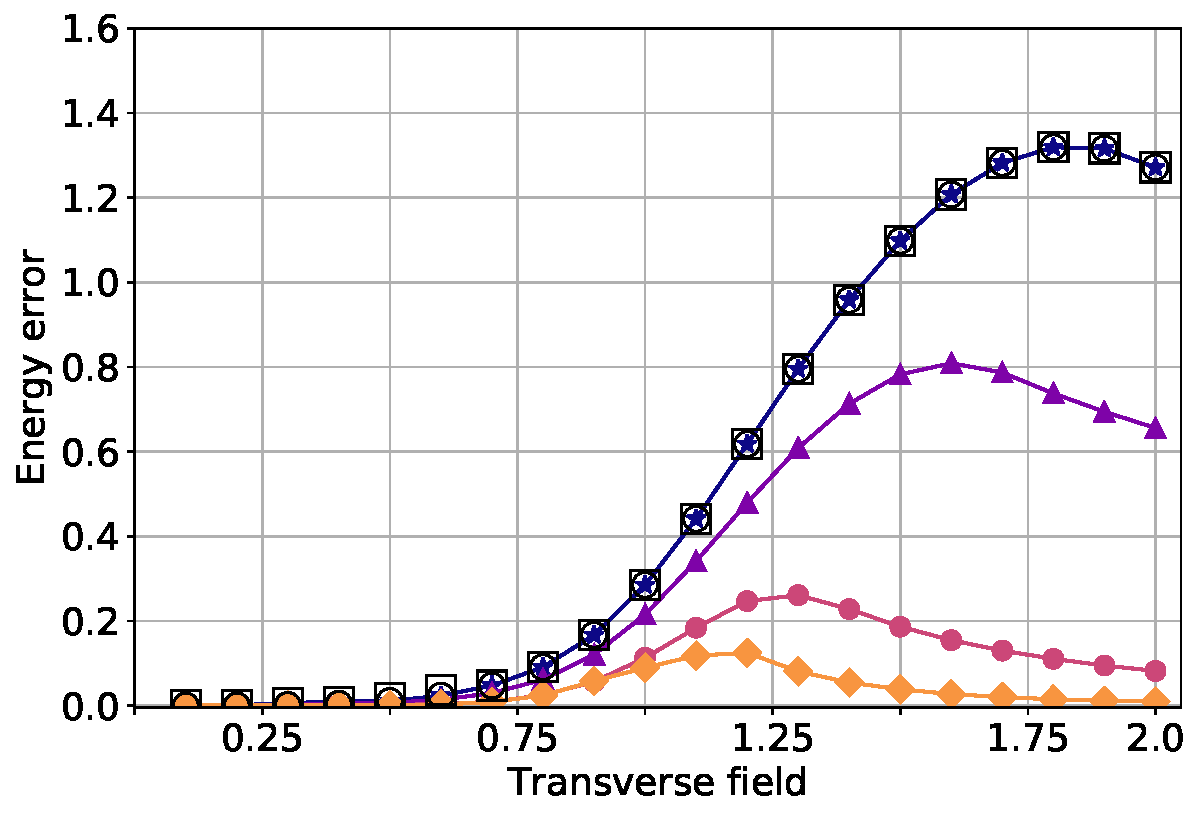
\includegraphics[width=0.7\textwidth]{../figures/dE_ising.pdf}
    \caption{Absolute value of the difference in energy between the exact solution and VQE solutions for the transverse field Ising model. Hollow squares: rank-1 ansatz, hollow circles: tree tensor network, filled markers: checkerboard states ($\bigstar$: 1 layer, $\blacktriangle$: 2 layers, $\bullet$: 3 layers, $\blacklozenge$: 4 layers). Reprinted from \cite{uvarov_machine_2020}.}
    \label{fig:dE_ising}
\end{figure}

The second model considered in this section is the Heisenberg XXZ model:

\begin{equation}
    \label{eq:heisenberg_xxz}
    H = \sum_{i=1}^n \left[J_\perp\left(X_i X_{i+1} + Y_i Y_{i+1}\right)
        + J_z Z_i Z_{i+1}\right].
\end{equation}

For this model, the error dependence was studied using the best ansatz among those studied for the TFI model. The solutions obtained using AAVQE were found to exhibit different behavior depending on the direction of movement through the parameter range (Fig.~\ref{fig:dE_xxz}).

\begin{figure}
    \centering
    \begin{subfigure}{.48\linewidth}
        \centering
        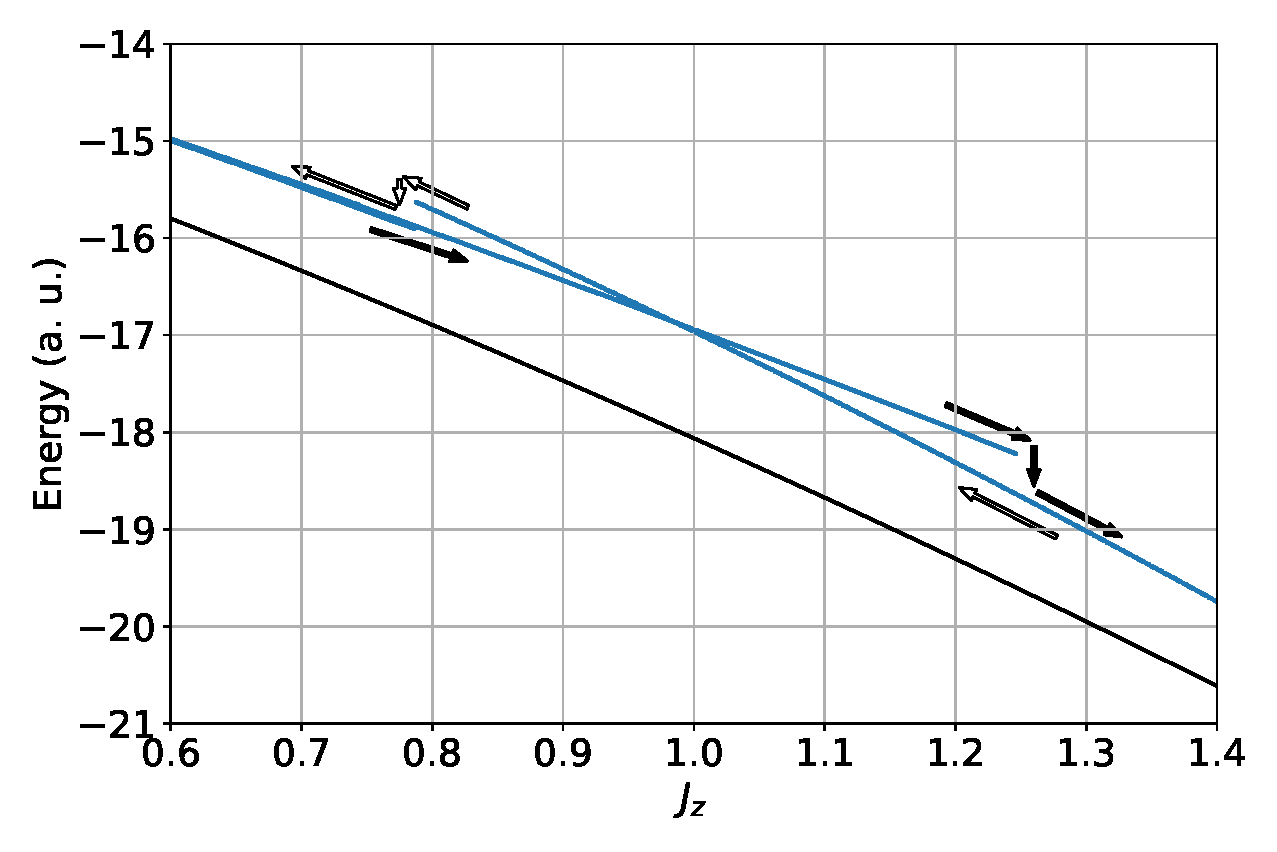
\includegraphics[width=\textwidth]{../figures/vqe_hysteresis_xxz_new.eps}
    \end{subfigure}\begin{subfigure}{.48\linewidth}
        \centering
        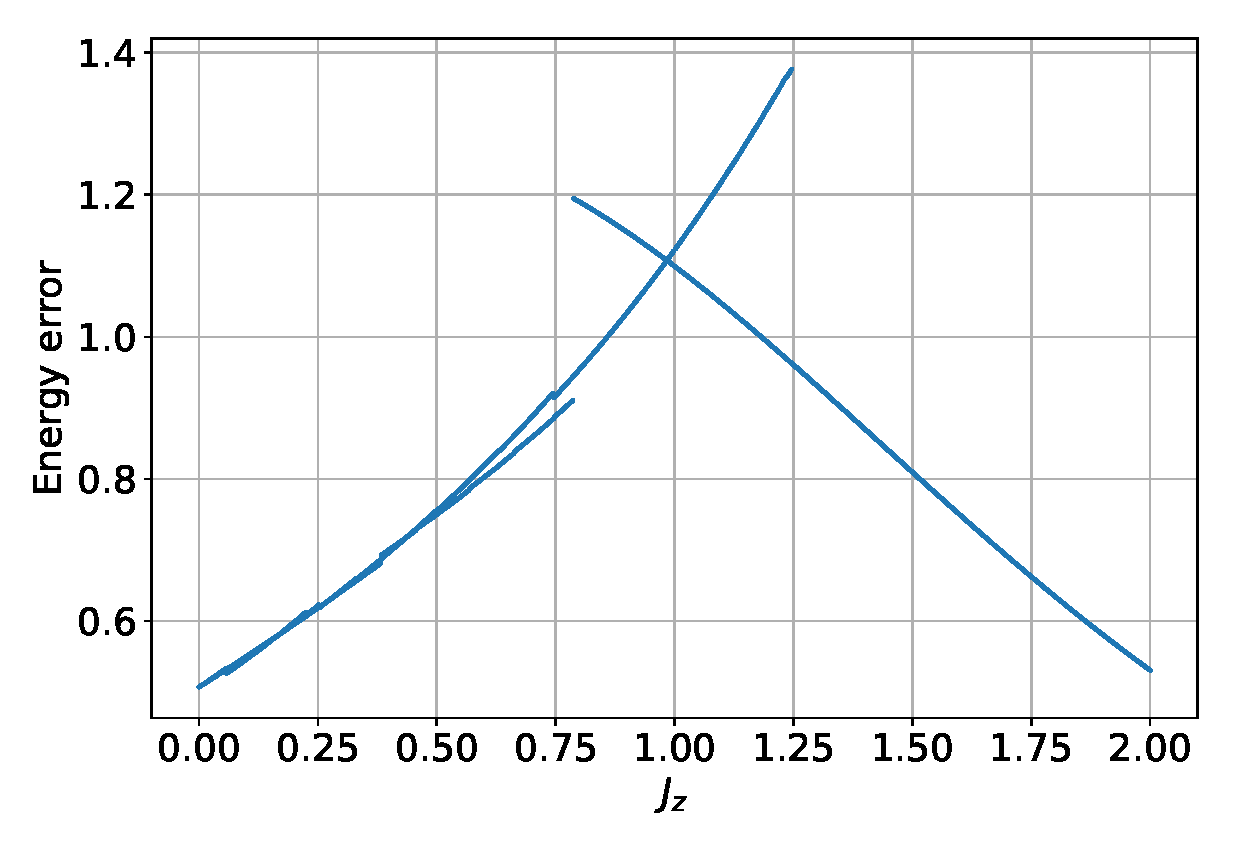
\includegraphics[width=\textwidth]{../figures/dE_xxz_best.eps}
    \end{subfigure}
    % 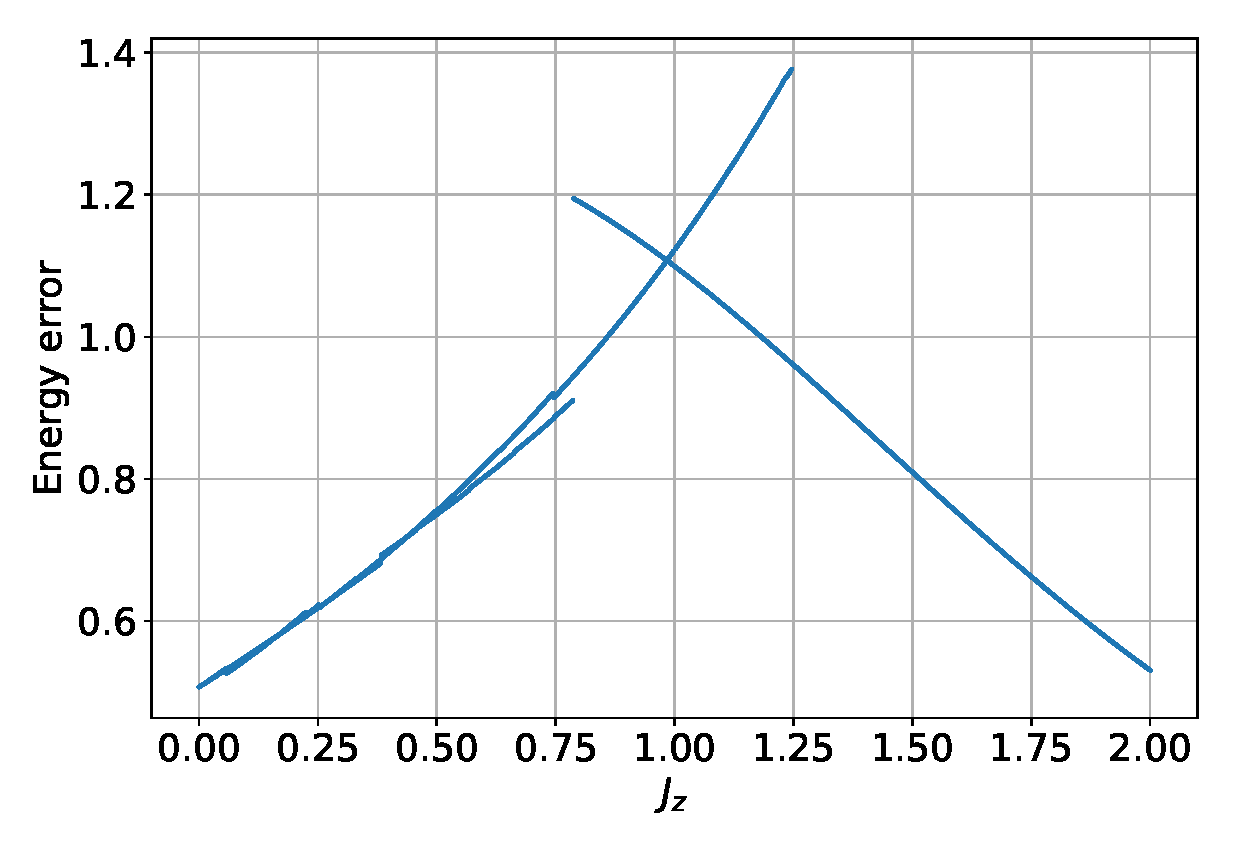
\includegraphics[width=0.7\textwidth]{../figures/dE_xxz_best.eps}
    \caption{Left: Ground-state energy estimate for the XXZ model found
    in VQE sweeps. Filled (empty) arrows guide the eye along the
    “up” (“down”) sweep. The black line denotes the energy of the exact solution. Reprinted from \cite{uvarov_machine_2020}. Right: Energy difference between the exact solution and the ansatz solutions for the XXZ model.}
    \label{fig:dE_xxz}
\end{figure}

Section 3.3 presents the results of simulating VQE for the Hubbard model. This model describes the behavior of fermions on a one-dimensional chain of sites, governed by Coulomb repulsion:

\begin{equation}
    H_{\text{Hubbard}} = \sum_{i \in [n], \sigma \in \{\uparrow, \downarrow\}} \epsilon_{i \sigma} \hat{n}_{i \sigma}
    - \sum_{<i, j>, \sigma \in \{\uparrow, \downarrow\}} t_{ij, \sigma} (a^\dagger_{i \sigma} a_{j \sigma} + a^\dagger_{j \sigma} a_{i \sigma})
    + U \sum_{i \in [n]} \hat{n}_{i \uparrow} \hat{n}_{i \downarrow},
\end{equation}

Our numerical experiments consider a simplified model, in which every site accommodates only one particle, and all particles are spinless. On the other hand, the Coulomb repulsion is extended to nearest-neighbor and next-nearest-neighbor sites:
\begin{equation}
    \label{eq:hubbard_nnn}
    H = - \sum_{<i, j>} t_{ij} (a^\dagger_{i} a_{j} + a^\dagger_{j} a_{i})
    + \sum_{i, j} U_{ij} \hat{n}_{i} \hat{n}_{j}.
\end{equation}
Here $t_{ij} = 1, U_{i, i+1} = V_1, U_{i, i+2} = V_2$, and all other terms $U_{ij}$ are zero.

The Hamiltonian was mapped to a spin Hamiltonian using the Jordan--Wigner transform. The numerical experiments use the checkerboard ansatz with two-qubit blocks preserving the number of particles \cite{barkoutsos_quantum_2018}:

\begin{equation}
\label{eq:particle-conserving_gate}
    U(\theta_1, \theta_2) = 
    \begin{pmatrix}
1 & 0 & 0 & 0 \\
0 & \cos{\theta_1} & e^{\imath \theta_2} \sin \theta_1 & 0 \\
0  & e^{-\imath \theta_2} \sin \theta_1  & -\cos{\theta_1} & 0  \\
0 & 0 & 0 & 1
\end{pmatrix}.
\end{equation}

Figure \ref{fig:vqe_hubbard_nnn} shows the results of VQE optimization for the model (\ref{eq:hubbard_nnn}) for different numbers of qubits and depths of the circuit. For the most part, the energy exhibits exponential convergence with the depth of the ansatz circuit, although the exact value of the exponent is different for different numbers of qubits. The jagged appearance of the curves is due to the fact that the specific particle-conserving gate used in the ansatz does not possess the identity gate in its configuration space. It is also clear that for larger $n$, the convergence tends to go slower. In particular, for $n=11$ qubits, the energy error remains roughly the same despite the increase in the number of layers.

\begin{figure}
    \centering
    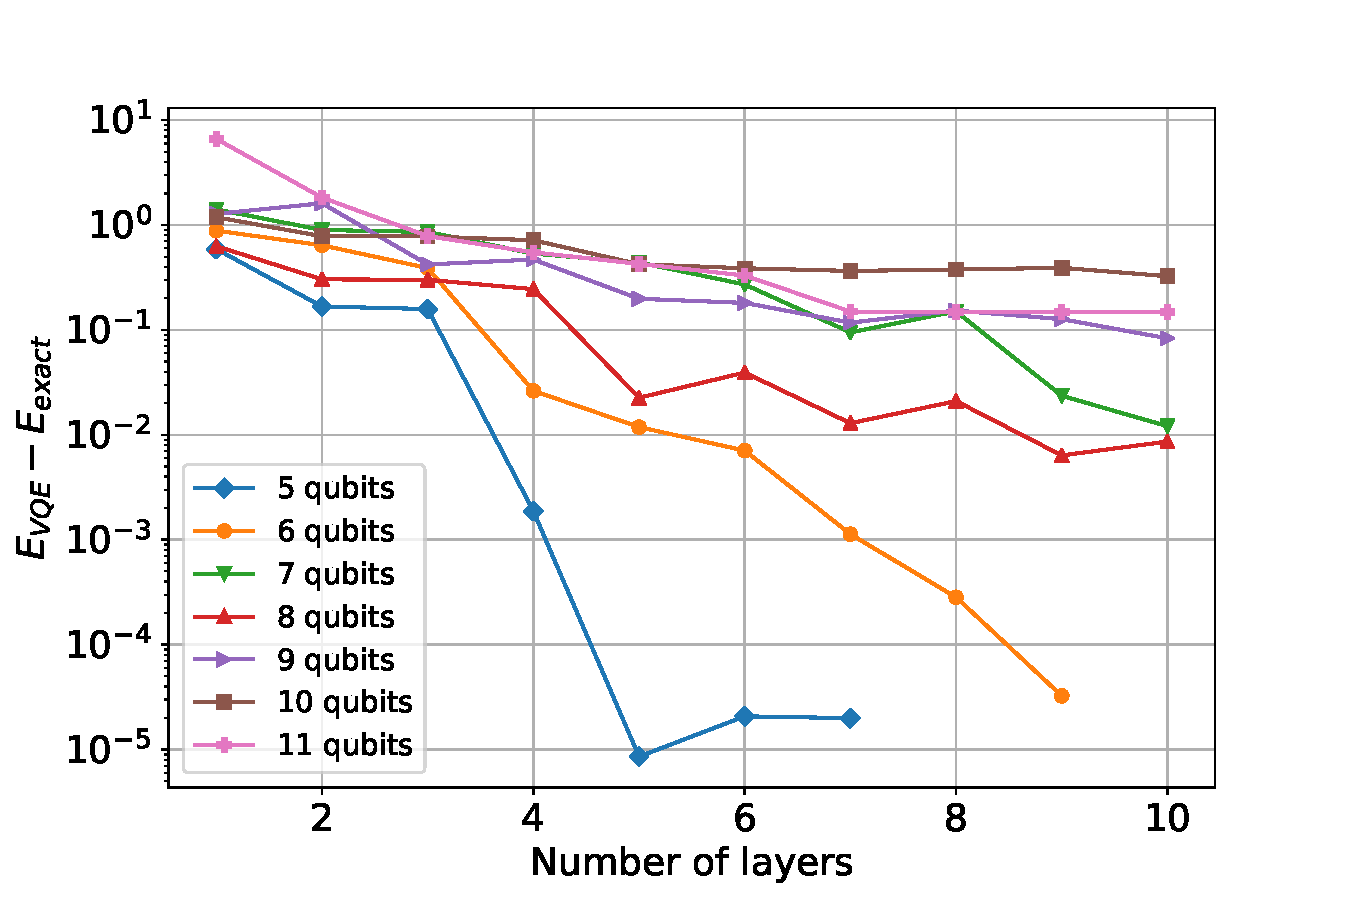
\includegraphics[width=0.7\textwidth]{../figures/vqe_hubbard_nnn.pdf}
    \caption{Convergence of the VQE solution to the true ground state for the 1D next-nearest-neighbor repulsion Hubbard model versus the number of layers, on condition $V_1 = 2t, V_2 = t$. Cases of $n \leq 4$ qubits are not shown as they converged to exact solution within 2 layers. Reprinted from \cite{uvarov_variational_2020}.}
    \label{fig:vqe_hubbard_nnn}
\end{figure}

In addition to the energy error of the numerical solutions, we studied the behavior of correlation functions. The results are shown in Fig.~\ref{fig:correlation}. While the qualitative agreement is evident, the accuracy of the approximation, as well as the size of the spin chain, were too low to produce any reasonable quantitative estimates of the asymptotical behavior of the correlation function.

\begin{figure}
    \centering
    \includegraphics*[width=0.7\textwidth]{../figures/Correlation.pdf}
    \caption{Density-density correlation function between spatially separated lattice sites. Filled dots denote exact values as obtained by virtue of exact diagonalization of the Hamiltonian (\ref{eq:hubbard_nnn}), dashed lines denote different approximations. Here $V_1 = 2t, V_2 = t$. Reprinted from \cite{uvarov_variational_2020}.}
    \label{fig:correlation}
\end{figure}

The final part of the section is devoted to studying the occurrence of the barren plateaus effect for the Hubbard model. The barren plateaus effect is an observation regarding the cost function landscape in variational quantum algorithms. For a sufficiently deep and expressive ansatz circuit, the derivative of the cost function becomes vanishingly small. Specifically, under the random choice of ansatz parameters, the expected value of all partial derivatives is zero, and the variance is exponentially small in the number of qubits $n$ \cite{mcclean_barren_2018}. This result, however, concerns very long circuits. The transient behavior of the derivatives is studied in this section.

Figure \ref{fig:plateaus_hubbard_ising}, top left, shows the behavior of the variance of the derivatives (averaged over random selections of $\boldsymbol{\theta}$ and $k$) for the next-nearest-neighbor Hubbard model (\ref{eq:hubbard_nnn}) under the Jordan--Wigner mapping. The particle-conserving ansatz is used for the analysis. For most qubit numbers and regardless of the model parameters, said variance drops to its limiting value even for very shallow circuits. In contrast, the same derivatives under the Bravyi--Kitaev mapping show a more gradual behavior (Figure \ref{fig:plateaus_hubbard_ising}, top right): the variance starts off by decaying exponentially with the depth, then saturates. The particle-preserving gate in the ansatz was replaced with a more generic gate, since the former would no longer conserve the particle number.
For comparison, we also performed a similar experiment for the transverse field Ising model. The gradient behavior away from the critical point ($h = 0.1$) and at the critical point ($h = 1$) is shown in Fig.~\ref{fig:plateaus_hubbard_ising}, bottom. In this case, the gradient variance decays exponentially with the number of layers until reaching the plateau regime for the particular number of qubits. Thus, for 4 qubits the plateau is reached right away, while for 10 qubits, 30 layers of the ansatz are still a number belonging to the transition regime. In the meantime, the criticality of the model does not seem to affect this behavior. A possible reason for the behavior observed in these three cases is that the Jordan--Wigner mapping produces highly nonlocal operators which are difficult to optimize.

\begin{figure}
    \centering
    \begin{subfigure}{.48\linewidth}
        \centering
        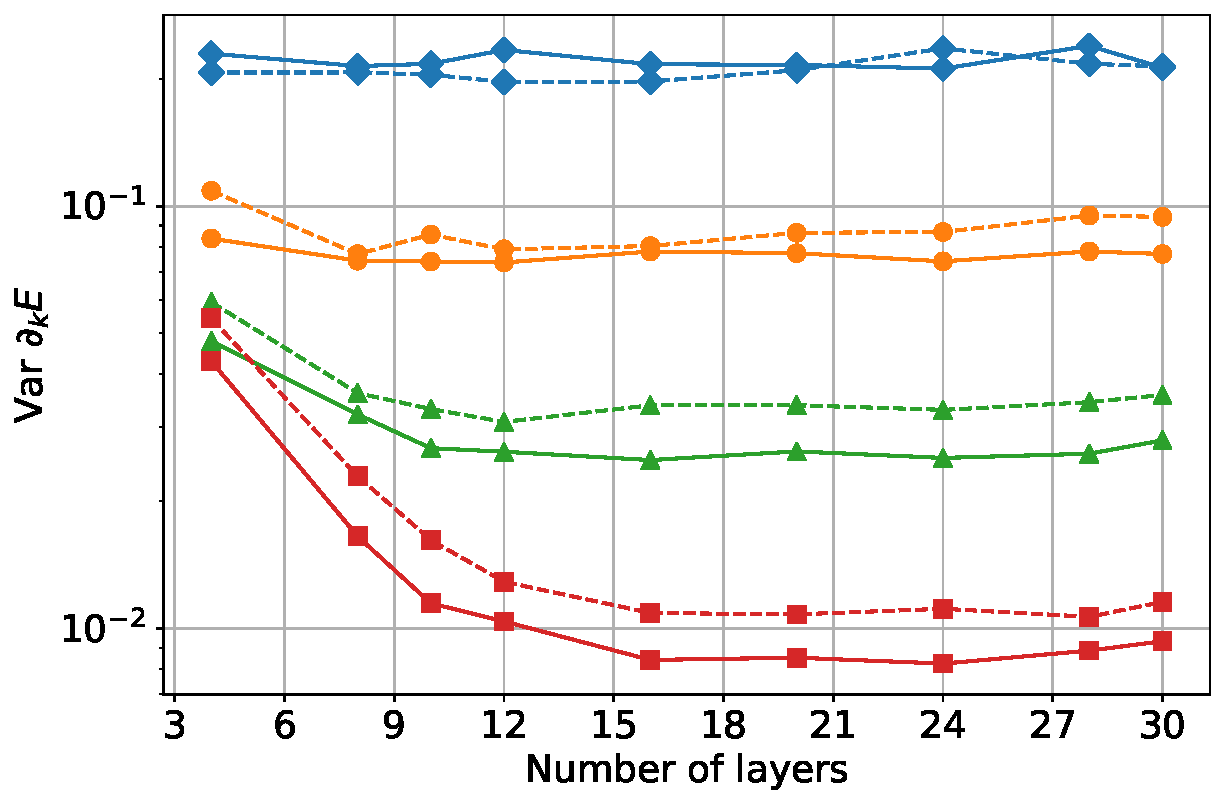
\includegraphics[width=\textwidth]{../figures/plateau_hubbard_jw_both.pdf}
    \end{subfigure}\begin{subfigure}{.48\linewidth}
        \centering
        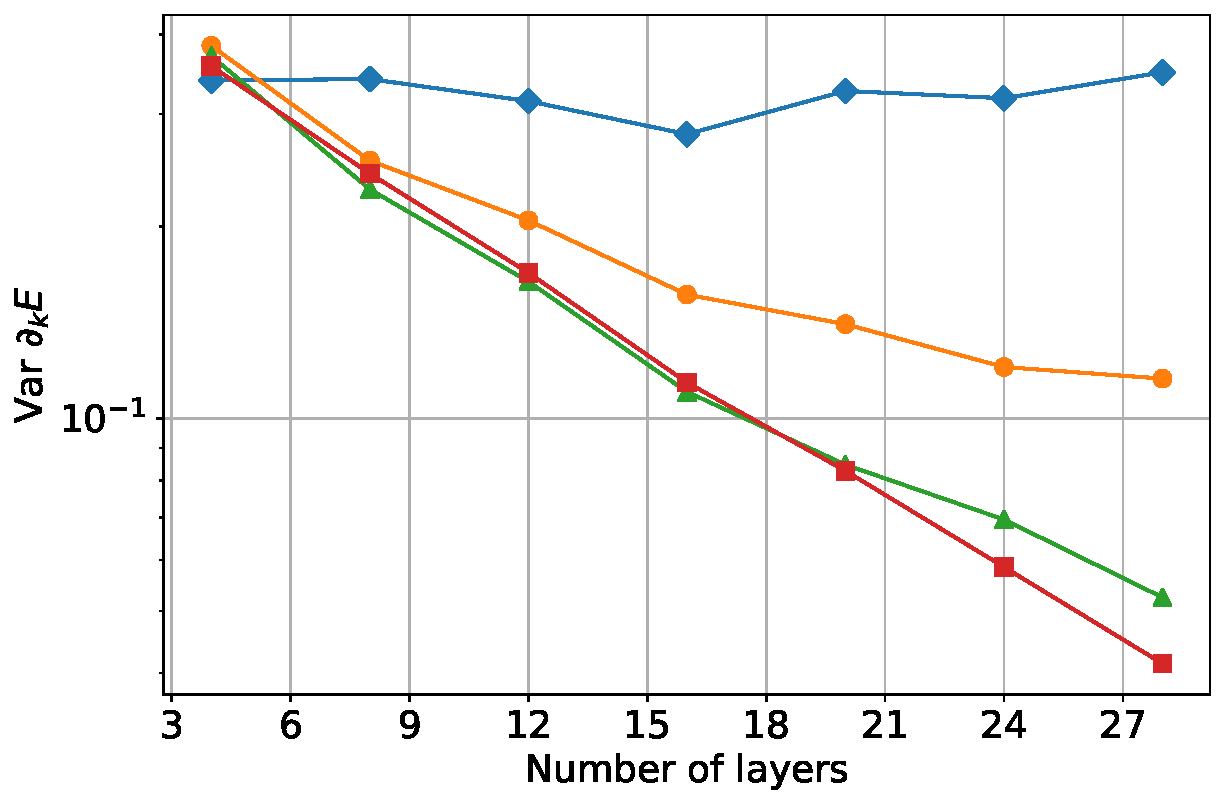
\includegraphics[width=\textwidth]{../figures/plateau_hubbard_bk.pdf}
    \end{subfigure}
    \begin{subfigure}{.48\linewidth}
        \centering
        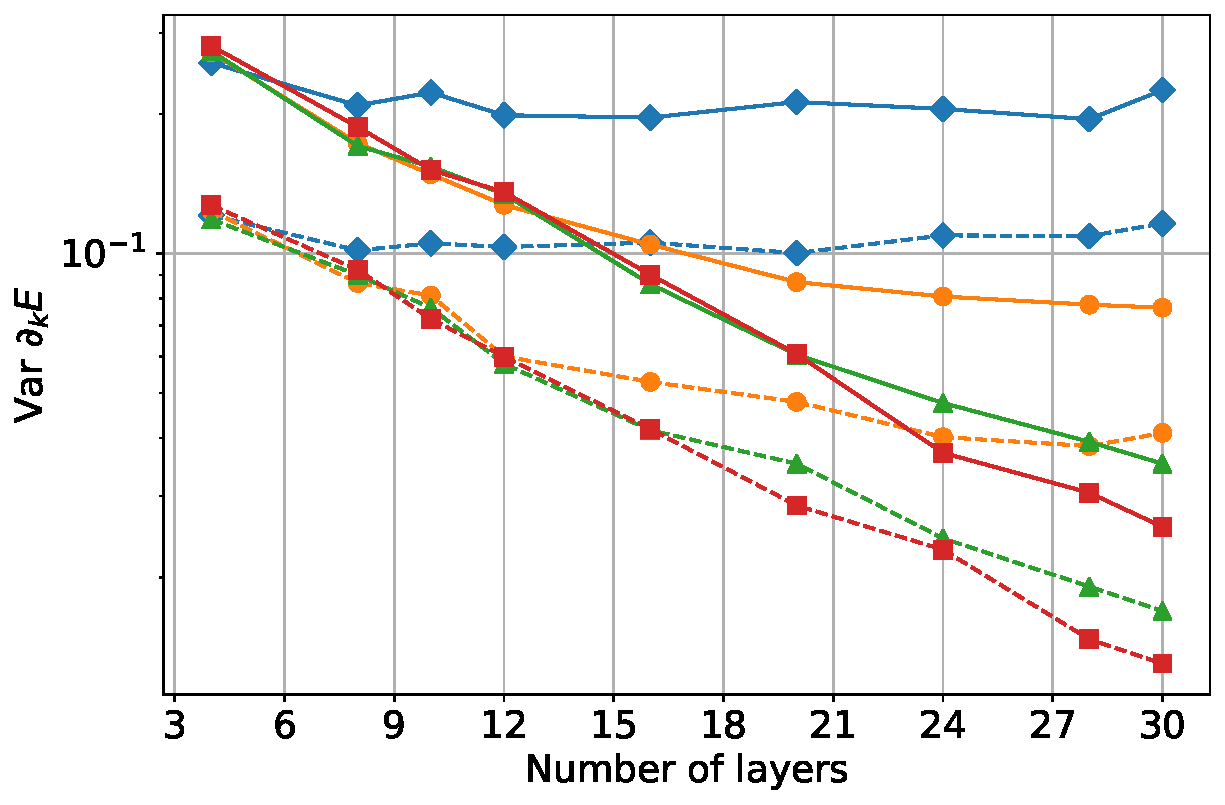
\includegraphics[width=\textwidth]{../figures/plateau_ising_both.pdf}
    \end{subfigure}
    \caption{\textbf{Top left:} barren plateau effect for the Hamiltonian of Eq. (3) with
    $V_1 = t$ and $V_2 = 0$ (dashed lines), as well as $V_1 = 2t$ and $V_2 = t$
    (solid lines) versus the number of qubits as realized by virtue of
    Jordan--Wigner mapping. Diamonds: four qubits; circles: six qubits;
    triangles: eight qubits; squares: 10 qubits. \textbf{Top right:} same effect under Bravyi--Kitaev mapping, $V_1 = 2t$, $V_2 = t$.
    \textbf{Bottom:} same effect for for the transverse field Ising model of Eq. (4) away from criticality with $h = 0.1$ (dashed lines) and at the critical point $h = 1$ (solid lines).    
    Reprinted from \cite{uvarov_variational_2020}.}
    \label{fig:plateaus_hubbard_ising}
\end{figure}

Section 3.4 contains concluding remarks. 

\textbf{The fourth chapter} discusses the possibility of applying VQAs to machine learning problems. Section 4.1 introduces the quantum approach to machine learning and reviews the existing literature on the topic. Section 4.2 presents our results in training a quantum classifier on quantum data obtained from VQE experiments. We start with the TFI model studied in the third chapter. This model has a phase transition point at $h=1$. Thus, the solutions obtained by VQE can be partitioned in two subsets: those for $h<1$ and those for $h>1$. The task of the classifier was to distinguish between these two classes.

\begin{figure}
    \centering
    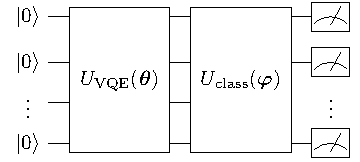
\includegraphics[width=0.7\linewidth]{../figures/classifier_circuit.pdf}
    \caption{Quantum circuit that implements the classifier. The first part prepares the VQE solution, the second one performs the classification. The assigned label is inferred from the measurements in the $Z$ basis. Both $U_{\mathrm{VQE}}$ and $U_{\mathrm{class}}$ have the checkerboard structure. Reprinted from \cite{uvarov_machine_2020}.}
    \label{fig:classifier_scheme}
\end{figure}

The classifier of quantum states is again a variational quantum circuit $U_{\mathrm{class}}$. The overall circuit is then the concatenation of the circuit preparing VQE solutions and the classifier circuit (Fig.~\ref{fig:classifier_scheme}). The label assigned by the neural network is proportional to the amount of qubits measured in the state ``1'', i.e.~the signal is the majority vote of the qubits. Effectively, estimating the majority is equivalent to estimating the energy of the state $U_{\mathrm{class}}(\boldsymbol{\varphi}) \ket{\psi(\boldsymbol{\theta})}$ relative to the following Hamiltonian:
\begin{equation}
    \label{eq:h_vote}
    H_{\text{vote}} = \sum_{w(i) > n/2} \ket{i} \bra{i} + \frac{1}{2}\sum_{w(i) = n/2} \ket{i} \bra{i}.
\end{equation}
Here $w(i)$ denotes the Hamming weight of the basis state $\ket{i}$, i.e.~the number of ones it contains.

To train the classifier circuit $U_{\mathrm{class}}(\boldsymbol{\varphi})$, we used the log-likelihood cost function. Let $\{ (\boldsymbol{\theta}_i, y_i) \}_{i=1}^{N_{train}}$ be the set of training data points and their labels, $y_i \in \{0, 1\}$. Let $p_i \in [0, 1]$ be the label predicted by the neural network:
\begin{equation}
    p_i = \bra{\psi(\boldsymbol{\theta}_i)} U^\dagger_{\mathrm{class}} (\boldsymbol{\varphi})H_{\text{vote}} U_{\mathrm{class}}(\boldsymbol{\varphi})\ket{\psi(\boldsymbol{\theta}_i)}.
\end{equation}
Then the loss function is:
\begin{equation}
\label{eq:logloss}
    f = -\sum_{i=1}^{N_{train}} \left( y_i \log p_i + (1 - y_i) \log (1 - p_i) \right).
\end{equation}
The classifier was successfully trained to distinguish the phases in the TFI model with 97\% accuracy (Fig.~\ref{fig:phase_classification}, left).

The next part of the section reports the same experiment for the Heisenberg XXZ model (\ref{eq:heisenberg_xxz}). This model also has a phase transition point at $J_z = 1$, $J_\perp = 1$, however in this case, it is more complicated to detect. As a result, the classifier circuit has to be extended by 2 layers. Another complication comes from the rotational symmetry of the model. Nonetheless, the classification was still performed successfully, albeit at a lower accuracy of 93\% (Fig.~\ref{fig:phase_classification}, right). 

The final paragraph of the section presents the test of the classifier on a model constructed by using two random Hamiltonians: $H(\alpha) = (1 - \alpha) H_1 + \alpha H_2, \ \alpha \in [0, 1]$, where $H_1$ and $H_2$ are random Hermitian matrices sampled from the Gaussian unitary ensemble. We split solutions in two classes: (i) $\alpha < 0.5$ and (ii) $\alpha > 0.5$. Then we run the optimization routine to train the learning circuit to discern between the two  classes. The accuracy in this experiment reached 93\%.


\begin{figure}
    \centering
    \begin{subfigure}{.48\linewidth}
        \centering
        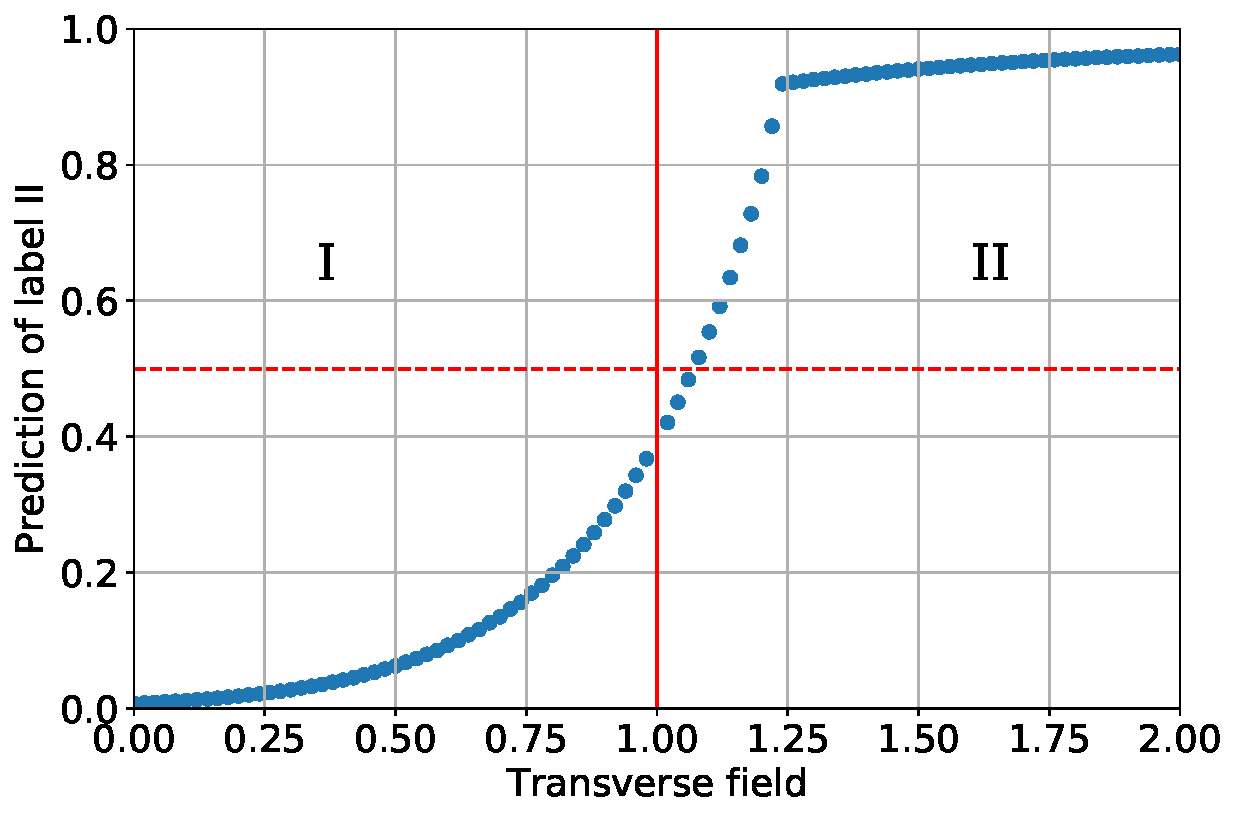
\includegraphics[width=\textwidth]{../figures/tfi_classification_new_2021}
    \end{subfigure}\begin{subfigure}{.48\linewidth}
        \centering
        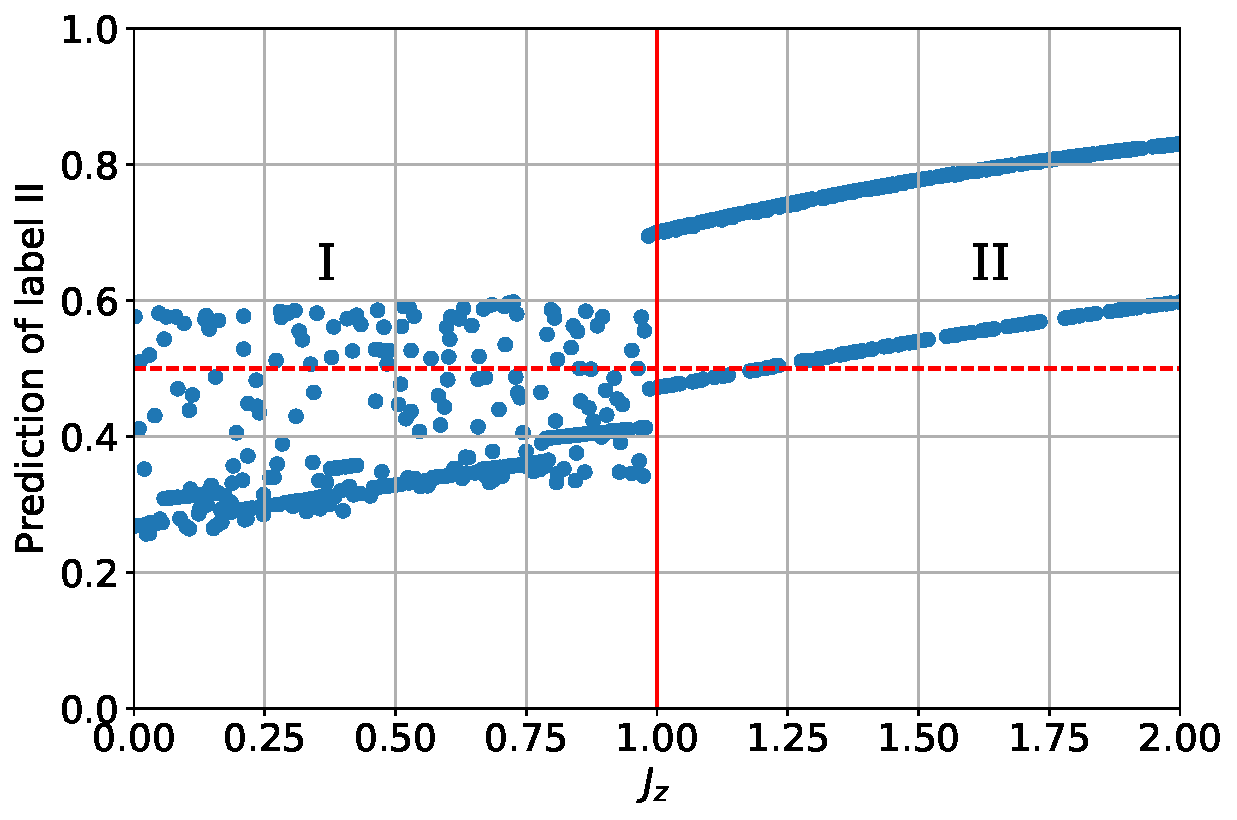
\includegraphics[width=\textwidth]{../figures/xxz_classification_new_2021.pdf}
    \end{subfigure}
    \caption{Left: predicted label of phase II as a function of magnetic field for transverse field Ising model. Right: predicted label of phase II as a function of $J_z$ for the XXZ model. Roman numbers denote the phases I and II of the models.}
    \label{fig:phase_classification}
\end{figure}

Section 4.3 discusses the possible alternative setups in quantum classification. One modification of the protocol is called learning by confusion: when we don't know the location of the phase transition point, we partition the examples with respect to a guess point $h^*$, then compare the results for different values of $h^*$ and pick the one with the best test accuracy \cite{van_nieuwenburg_learning_2017}. We present a simple test of that approach and observe that it successfully predicts the phase transition point. Another important choice in the setup is the cost function. We discuss measuring just the first qubit as a possible alternative. The conclusions of the chapter are given in Section 4.4.

\textbf{The fifth chapter} presents our the results of our study of the barren plateaus phenomenon, previously encountered in the third chapter. Section 5.1 introduces the Haar measure and integration with respect to it. 
\begin{definition}
    The \textit{Haar measure} $\mu: \mathrm{Borel} (U(d)) \rightarrow [0, 1]$ on the unitary group $U(d)$ is the unique left- and right-invariant probability measure on that group. That is, let $V \in U(d)$ and let $\mathcal{A} \in \mathrm{Borel} (U(d))$. Then $\mu(\mathcal{A}) = \mu(V \mathcal{A}) = \mu(\mathcal{A} V)$.
\end{definition}
The main results presented in this section are two integrals over the Haar measure:
\begin{equation}
    \label{eq:haar_integral_1}
    \int U^\dagger A U \mathrm{d} \mu = \frac{\operatorname{Tr} A}{d} \cdot I
\end{equation}
\begin{align}
    \label{eq:haar_integral_2}
     \int (U^\dagger \otimes U^\dagger) (A \otimes B) (U \otimes U) \mathrm{d} \mu & = 
      \frac{1}{d^2 - 1} \left[  
         (\Tr A \Tr B  - \frac{1}{d} \Tr AB) \mathbbm{1} \otimes  \mathbbm{1} + \right. \\
       &  \left. + (\Tr AB  - \frac{1}{d} \Tr A \Tr B) \mc{S} \right].
\end{align}
Here $A, B \in \operatorname{End}(\mathbb{C}^d)$ are arbitrary linear operators, and $\mc{S}$ denotes a swap of two tensor components: $\mc{S} (v \otimes w) = w \otimes v$.

Section 5.2 introduces the $t$-designs, which are unitary ensembles that mimic the lowest moments of the Haar distribution while possibly being easier to sample from.
\begin{definition}
    A probability distribution $\nu$ on the unitary group $U(2^n)$ is a  \textit{unitary} $t$\textit{-design}
    if the expected value of any polynomial of power $t$ in the matrix elements of $U$ and $U^*$ with respect to $\nu$ is the same as that w.r.t.~the Haar measure on $U(2^n)$.  
\end{definition}
We also introduce so-called \textit{approximate $t$-designs} and \textit{tensor product expanders}. There are many definitions for different purposes \cite{low_pseudo-randomness_2010}, but we picked those that we found the most convenient for a numerical experiment.
\begin{definition}
    An ensemble of random unitary gates $\nu$ is a $\lambda$-approximate tensor product expander (TPE) if $||\mathbb{E}_{Haar} (U^{\otimes t} \otimes (U^*)^{\otimes t}) - \mathbb{E}_\nu (U^{\otimes t} \otimes (U^*)^{\otimes t}) ||_p \leq \lambda$ for $p=\infty$. When such an equation holds for $p=1$, the ensemble $\nu$ is called a $\lambda$-approximate $t$-design.
\end{definition}
Section 5.3 formally introduces the barren plateaus phenomenon. We consider a parametrized quantum circuit in which we distinguish one gate: $U = U_A e^{-\mathrm{i} \theta F} U_B$, where $F$ is a Pauli string. Let our cost function be some local Hamiltonian $H = \sum c_i h_i$, where $h_i$ are Pauli strings, and $h_0 = I$. The energy to be minimized in VQE is then equal to 

\begin{equation}
    E = \bra{\psi_0} U_B^\dagger e^{\mathrm{i} \theta F} U_A^\dagger H U_A e^{-\mathrm{i} \theta F} U_B \ket{\psi_0}.    
\end{equation}

The energy derivative over $\theta$ is now equal to 

\begin{multline}
    \label{eq:partial_E}
    \partial_\theta E = \bra{\psi_0} U_B^\dagger e^{\mathrm{i} \theta F} (\mathrm{i} F) U_A^\dagger H U_A e^{-\mathrm{i} \theta F} U_B \ket{\psi_0} + \\
    +
    \bra{\psi_0} U_B^\dagger e^{\mathrm{i} \theta F} U_A^\dagger H U_A (-\mathrm{i} F) e^{-\mathrm{i} \theta F} U_B \ket{\psi_0} = \\
    = \mathrm{i} \bra{\psi_0} U_B^\dagger e^{\mathrm{i} \theta F}  [F, U_A^\dagger H U_A] e^{-\mathrm{i} \theta F} U_B \ket{\psi_0}.
\end{multline}

In this setup, the phrase ``barren plateaus'' refers to the following theorem, which is proven in the remainder of the section:

\begin{theorem}[after \cite{mcclean_barren_2018}]
    \label{thm:mcclean}
    Let either $U_A$ or $U_B$ form a $2$-design. If $\operatorname{card} H \in \operatorname{poly}(n)$, and the Pauli coefficients $c_i$ are bounded by a constant, then the variance $\operatorname{Var} \partial_\theta E \in O(2^{-n})$.
\end{theorem}

Section 5.4 reports on our theoretical contribution to the study of barren plateaus. We introduce the following definitions.

\begin{definition}[Super Pauli strings]
    If $h$ is a Pauli string, then we will call $h \otimes h$ the induced \emph{super Pauli string}. If a Pauli string acts on qubits labeled $1, 2, \dots, n$, then a super Pauli string acts on qubits labeled $1, 2, \dots, n, 1', 2', \dots, n'$.
\end{definition}

\begin{definition}[Causal cone] 
    Let $U$  be an ansatz, and $h$ a Pauli string. 
    A gate (or a block of gates) $V$ is in the \emph{causal cone} $C(h, U)$ of $h$ under ansatz $U$, if that gate or block cannot be eliminated from the conjugate $U^\dagger h U$. We denote as $|C(h, U)|$ the support of this causal cone, i.e.~the number of qubits on which $U^\dagger h U$ can act nontrivially.
\end{definition}


\begin{definition}[Mixer]

    Let $\mc{Y}$ be a subset of the qubit registry. Define the \textit{local mixing operator}, or simply a \textit{mixer}\footnote{The mixer is in fact a quantum channel since it is defined by its own Kraus decomposition.}  $M_{\mc{Y}}: \operatorname{End} (\mc{H}\otimes \mc{H}) \rightarrow \operatorname{End} (\mc{H}\otimes \mc{H})$ as follows:
    \begin{equation}
    \begin{aligned}
        \label{eq:m2}
        & M_{ \mc{Y}} (h_1 \otimes h_2) = \int d\mu_{\mc{Y}} (U)
        (U^\dagger \otimes U^\dagger)
        (h_1 \otimes h_2)
        (U \otimes U),
    \end{aligned}{}
    \end{equation}{}
    where $\mu_{\mc{Y}}$ is the Haar distribution of unitary operators acting nontrivially on $\mc{Y}$ and trivially on all other qubits.
    
\end{definition}

The mixer can act on super Pauli strings by conjugation. The results of this action are formulated in the following propositions.

\begin{proposition}
    \label{prop:m2_decomposed}
    Let $h$ be a Pauli string. If its substring $h_{\mc{Y}}$ is nontrivial, then
    
    \begin{equation}
        M_{\mc{Y}}(h \otimes h) = \frac{1}{4^{|\mc{Y}|} - 1} \left( \sum_{\sigma_\mc{Y} \neq \mathbbm{1}} (\sigma_{\mc{Y}} \otimes h_{\mc{H} \setminus \mc{Y}})^{\otimes 2}\right),
    \end{equation}{}
    where the summation extends over all nontrivial Pauli substrings $\sigma_{\mc{Y}}$.
    Otherwise,  $M_{\mc{Y}}(h \otimes h) = h \otimes h$.
    
\end{proposition}

\begin{proposition}
    \label{prop:mixer_kills_asymmetry}
    Let $h_1, h_2$ be Pauli strings such that their restriction on a registry $\mc{Y}$ is different. Then $\mc{M_Y} (h_1 \otimes h_2) = 0$.
\end{proposition}

\begin{proposition}
    \label{prop:paulis_decouple}
    Let $\mc{Y}_1, ..., \mc{Y}_N$ be a collection of qubit subsets
    such that $\mc{Y}_1 \cup ... \cup \mc{Y}_N$ contains all $n$ qubits (the subsets are allowed to intersect). Let $h_1, h_2$ be two distinct Pauli strings. Then, 
    $M_{ \mc{Y}_N} \circ \dots \circ  M_{ \mc{Y}_1} (h_1 \otimes h_2) = 0.$
\end{proposition}

Next, we introduce a commutator operator $\mc{C}_{F} \in \operatorname{End}(\mc{H} \otimes \mc{H})  \rightarrow \operatorname{End}(\mc{H} \otimes \mc{H})$, which maps $A \otimes B$ to $[\rmi F, A] \otimes [\rmi F, B]$. Unlike the mixer operator, $\mc{C}_F$ is no longer a quantum channel since it does not preserve trace. Graphically, we can express this superoperator like this:

\newcommand{\legw}{1}
\newcommand{\gapw}{2}
\newcommand{\gaph}{1}
\newcommand{\barh}{0.6}
\newcommand{\wireh}{0.2}
\newcommand{\wiregap}{0.5}
\newcommand{\wirel}{0.3}

\begin{equation}
    \mc{C}_F(\star) =
    \adjustbox{raise=-7pt}{
    \begin{tikzpicture}[thick,scale=0.5]
    \node[blank] at (\gapw/2 + \legw, \gaph/2) {$\star$};
    
    
    \draw 
    (0, 0) 
    -- (0, \gaph + \barh) 
    -- (\gapw + \legw + \legw,\gaph + \barh)
    -- (\gapw + \legw + \legw,0)
    -- (\gapw + \legw,0)
    -- (\gapw + \legw, \gaph)
    -- (\legw, \gaph)
    -- (\legw,0)
    -- (0, 0)
    
    (0, \wireh) -- (-\wirel, \wireh)
    (0, \wireh + \wiregap) -- (-\wirel, \wireh + \wiregap)
    
    (\legw, \wireh) -- (\legw + \wirel, \wireh)
    (\legw, \wireh + \wiregap) -- (\legw + \wirel, \wireh + \wiregap)
    
    (\legw + \gapw, \wireh) -- (\legw + \gapw - \wirel, \wireh)
    (\legw + \gapw, \wireh + \wiregap) -- (\legw + \gapw - \wirel, \wireh + \wiregap)
    
    (\gapw + \legw + \legw, \wireh) -- (\gapw + \legw + \legw + \wirel, \wireh)
    (\gapw + \legw + \legw, \wireh + \wiregap) -- (\gapw + \legw + \legw + \wirel, \wireh + \wiregap)
    
    ;
    \end{tikzpicture}
    }
\end{equation}

\begin{proposition}
    \label{prop:commutator_old}
    The following identities hold:
    \begin{enumerate}
        \item For every $F \in \mathrm{Herm}(\mc{Y})$, $\mc{C}_{F}(\id_{\mc{Y}} \otimes \id_{\mc{Y}})$ vanishes. Thus, $M_{\mc{Y}} \circ \mc{C}_F \circ M_{\mc{Y}} (\id_{\mc{Y}} \otimes \id_{\mc{Y}})=0$.
        \item Let $F$ be a nontrivial Pauli string acting on $\mc{Y}$. Then, for any nontrivial Pauli string $h$ acting on $\mc{Y}$
        \begin{equation}
            \label{eq:sandwiched_commutator}
             M_{\mc{Y}} \circ \mc{C}_{F} \circ M_{\mc{Y}} \left( h^{\otimes 2}\right) = \frac{2 \cdot 4^{|\mc{Y}|}}{4^{|\mc{Y}|} - 1} M\left( h^{\otimes 2}\right).
        \end{equation}
    \end{enumerate}{}
\end{proposition}{}

In subsection 5.4.2 we are ready to formulate the main statements of the chapter.

\begin{theorem}
    \label{thm:block_plateaus}
    Let $H$ be an $n$-qubit Hamiltonian consisting of Pauli strings $h_i$: $H = \sum c_i h_i$ with finite $c_i \in \mathbb{R}$. Let the ansatz $U$ consist of $l$ layers, and denote $l_c$ the layer which contains the block $G_k$ depending on parameter $\theta_a$. 
    % \textcolor{blue}{\textbf{[I don't think we should write $\theta_k$; a block typically depends on more than one parameter. Maybe we can highlight its special role in some other way, like $\tilde{\theta}$ or $\hat{\theta}$? --- Alexey]}}. 
    Let each block of the ansatz be an independently parametrized local 2-design. Let the block $G$ also be decomposable into $G = G_A e^{-i \theta_a F} G_B$, where $G_A$ and $G_B$ are local 2-designs not depending on $\theta_a$. Then, the variance of the gradient of $E$ with respect to that parameter is bounded below as follows:
    
    \begin{equation}
        \operatorname{Var} \partial_a E \geq \frac{2 \cdot 4^{|\mc{Y}_k|}}{4^{|\mc{Y}_k|} - 1} \left( \frac34 \right)^{l - l_c}  \sum_i c_i^2 \cdot 3^{-|C(h_i, U)|},
    \end{equation}{}
    where $|C(h_j, U)|$ is the number of qubits in the causal cone of the $j^{th}$ Pauli string, and the summation is over those Pauli strings whose causal cone contains the block $G$.
\end{theorem}{}

The proof of this theorem uses the fact that $\partial_a E (h_i)$ are uncorrelated random variables:

\begin{proposition}
\label{lemma:expectations_decouple}
In the conditions of Theorem \ref{thm:block_plateaus}, the individual Pauli string coefficients make independent contributions to the total variance:
\begin{equation}
    \operatorname{Var} \partial_a E (H) = \sum_i c_i^2 \operatorname{Var} \partial_a E (h_i).
\end{equation}
\end{proposition}

The rest of the section first offers a brief idea of the proof, then goes through the proof in detail.

\begin{figure}
    \centering
    \begin{subfigure}{.48\linewidth}
        \centering
        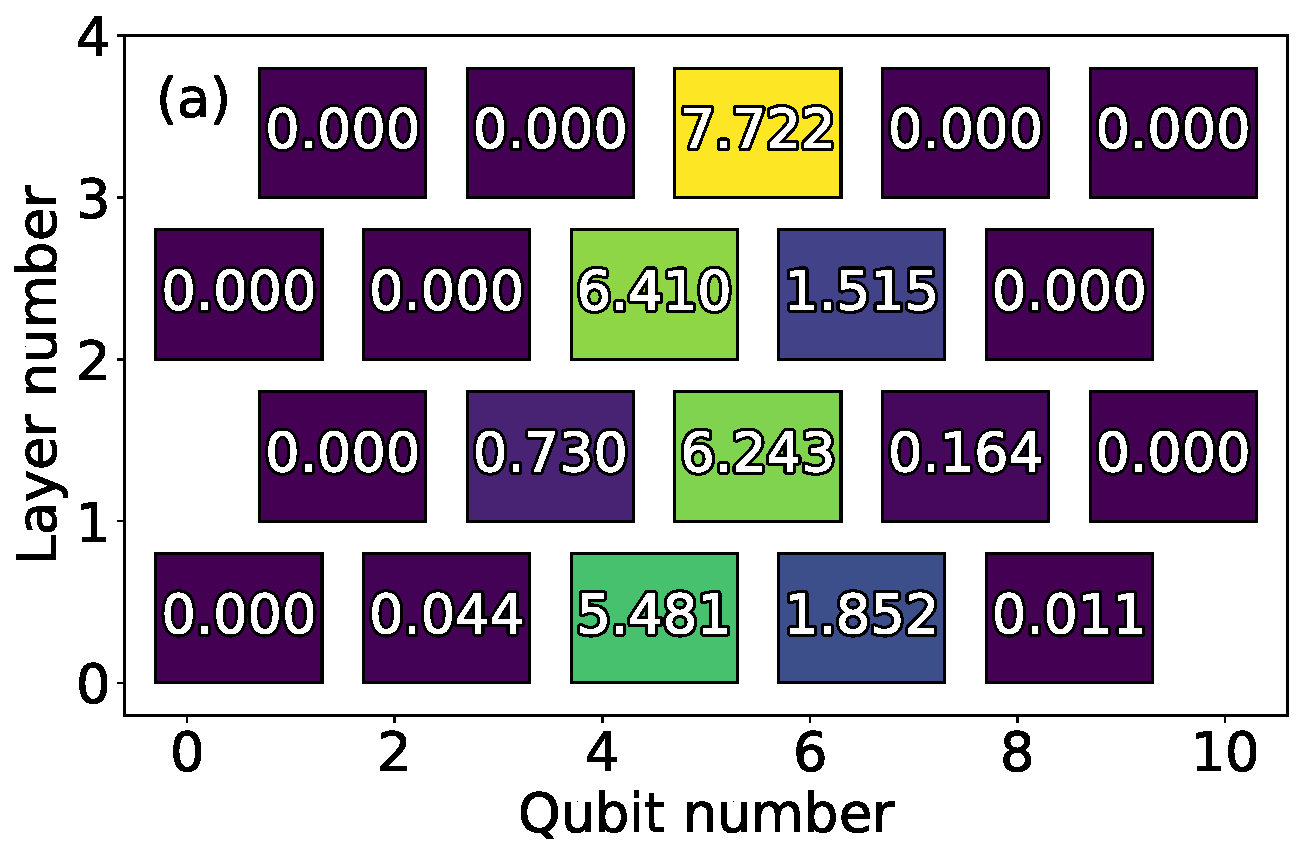
\includegraphics[width=\textwidth]{../figures/X5_ising.pdf}
    \end{subfigure}\begin{subfigure}{.48\linewidth}
        \centering
        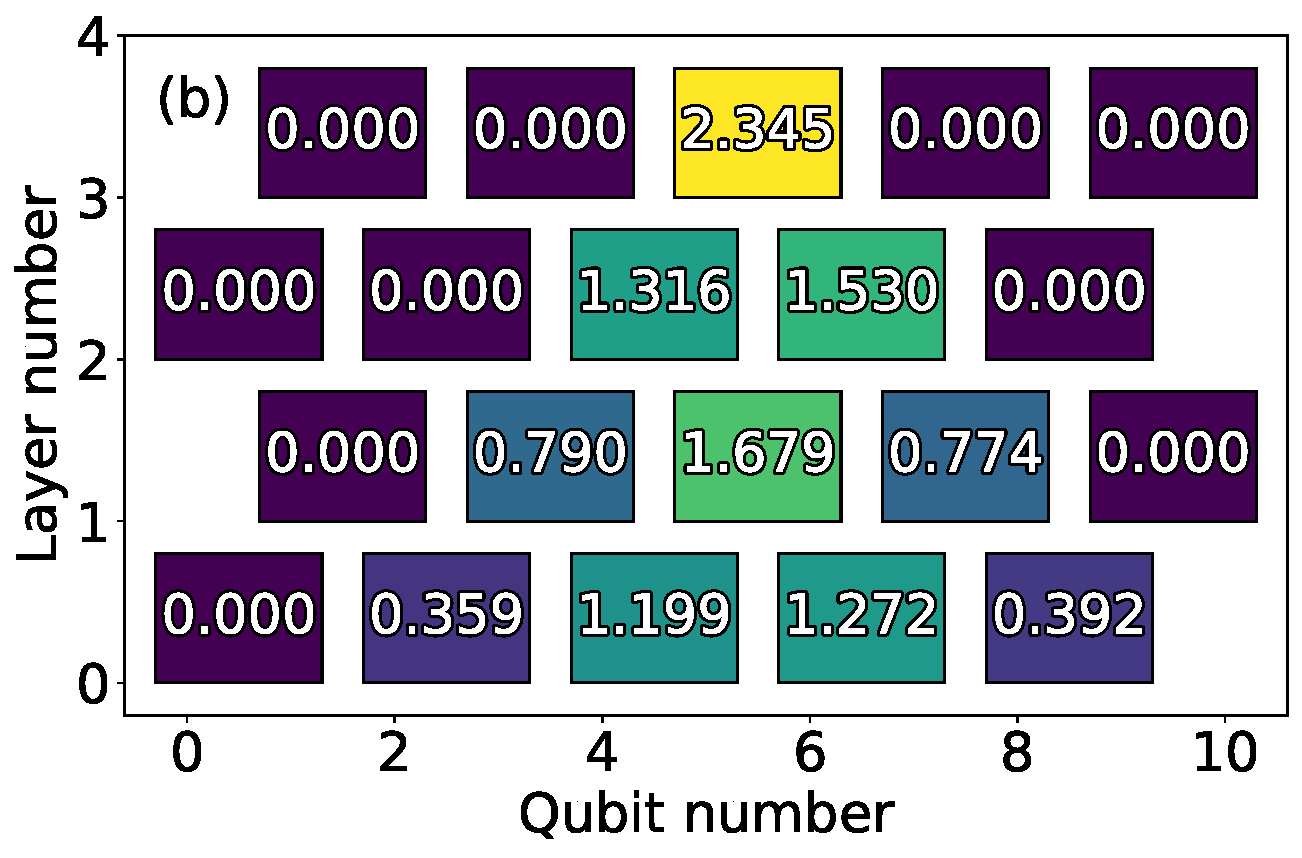
\includegraphics[width=\textwidth]{../figures/X5_cartan.pdf}
    \end{subfigure}
    \begin{subfigure}{.48\linewidth}
        \centering
        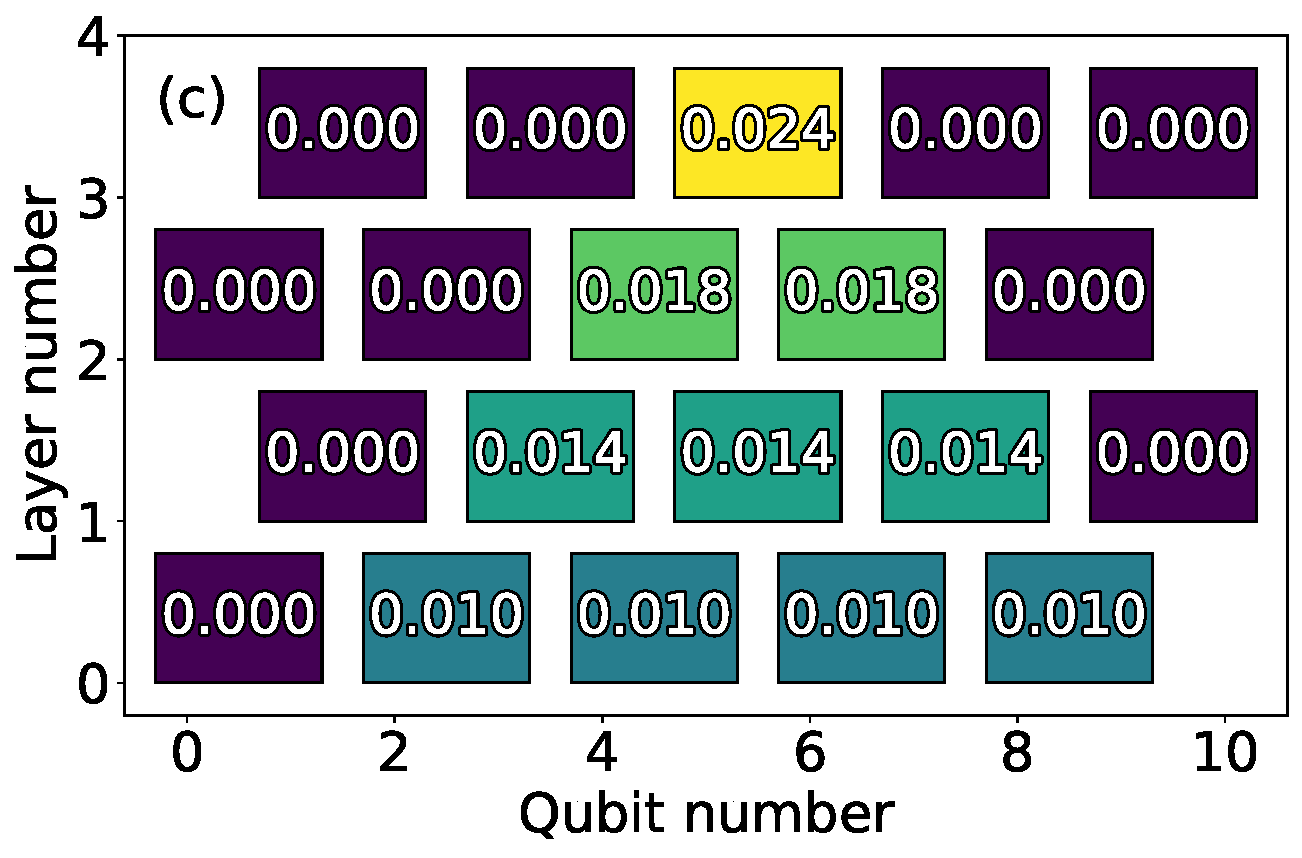
\includegraphics[width=\textwidth]{../figures/X5_theory.pdf}
    \end{subfigure}
    \caption{Derivative variances for $H = X_5$, averaged over parameters in each ansatz block. The numbers in the boxes denote $\Var \partial_\theta E \cdot 100$. Qubit number 10 is identified with qubit number 0. (a) Numerical result for an ansatz with blocks of $X,Z,ZZ$ rotations. (b) Numerical result for blocks implemented according to the Cartan decomposition. (c) Lower bound given in Theorem \ref{thm:block_plateaus}. Reprinted from \cite{uvarov_barren_2021}.}
    \label{fig:one-local}
\end{figure}

Section 5.5 presents numerical experiments supporting the main claims of the paper. The bound proven in Theorem \ref{thm:block_plateaus} holds in all cases considered, however it appears to be quite loose (e.g.~Fig.~\ref{fig:one-local}). The behavior of the derivatives also depends strongly on the choice of the blocks comprising the ansatz.
To justify the assumption that local circuit blocks are approximate 2-designs, we estimated their proximity by different norms. The results are shown in Table \ref{thm:block_plateaus}. 

\begin{table}
    \centering
    \begin{tabular}{|c|c|c|c|}
    \hline
        Block & 
        % Circuit diagram or matrix & 
        $\lambda_1$ & $\lambda_\infty$ & $\lambda_2$\\
        \hline
        $X$, $Z$, and $ZZ$ rotations &  
            % $\Qcircuit @C=1.0em @R=1.0em {
            %        \quad & \gate{R_Z} & \multigate{1}{R_{ZZ}} & \gate{R_X} & \qw \\
            %        \quad & \gate{R_Z} & \ghost{R_{ZZ}} & \gate{R_X} & \qw \\
            %    }$ &
        0.95 & 1.80 & 0.87\\
        \hline 
        Universal gates and a CNOT &
        %     $\Qcircuit @C=1.0em @R=1.0em {
        %    \quad & \gate{U_3} & \ctrl{1} & \gate{U_3} & \qw \\
        %    \quad & \gate{U_3} & \targ & \gate{U_3} & \qw \\
        %     }$
        % & 
        0.68 & 0.69 & 0.42\\
        \hline
        $Y$ rotations and a CZ \cite{cerezo_cost-function-dependent_2020} &            
        %     $\Qcircuit @C=1.0em @R=1.0em {
        %    \quad & \gate{R_Y} & \ctrl{1} & \gate{R_Y} & \qw \\
        %    \quad & \gate{R_Y} & \ctrl{-1} & \gate{R_Y} & \qw \\
        %     }$ 
            % & 
            1.76 & 1.76 & 1.00\\
        \hline
        Number-conserving \cite{barkoutsos_quantum_2018} & 
        % $
        % \begin{pmatrix}
        % 1 & 0 & 0 & 0 \\
        % 0 & \cos(\theta_1) & e^{i\theta_2} \sin(\theta_1) & 0 \\
        % 0 & e^{-i\theta_2} \sin(\theta_1) & -\cos(\theta_1) & 0 \\
        % 0 & 0 & 0 & 1 \\
        % \end{pmatrix}
        % $
        % & 
        2.40 & 2.40 & 1.00\\
        \hline
        Cartan decomposition \cite{khaneja_cartan_2000,khaneja_time_2001} &
    %     $\Qcircuit @C=1.0em @R=1.0em {
    %    \quad & \gate{U_3} & \multigate{1}{R_{XX}} & \multigate{1}{R_{YY}} & \multigate{1}{R_{ZZ}}& \gate{U_3} & \qw \\
    %    \quad & \gate{U_3} & \ghost{R_{XX}} & \ghost{R_{YY}} & \ghost{R_{ZZ}} & \gate{U_3} & \qw \\
    %     }$
    %         & 
            0.25 & 0.25 & 0.17\\
    \hline
    \end{tabular}
    \caption{Proximity to the 2-tensor product expander for different two-qubit blocks, estimated by random sampling. Circuit diagrams of ansatz blocks are given in the text of the dissertation.}
    \label{tab:local_designs}
\end{table}

Section 5.6 contains concluding remarks.

\textbf{The sixth chapter} proposes and analyzes a protocol for estimating the fidelity of Clifford states. Specifically, the chapter is focused on the Greenberger-Horne-Zeilinger (GHZ). This state is a popular target state for demonstration of all-to-all entanglement of qubits.
Section 6.1 reviews the techniques used in the literature to measure the fiedlity of the GHZ state: these methods involve measuring parity oscillations (PO) and multiple quantum coherences (MQC). 
Section 6.2 presents the mathematical tools required for the proposed method.

\begin{proposition}[Stability lemma]
    \label{prop:stability}
    Let $H$ be a Hamiltonian with eigenvalues $0 = \lambda_0 < \Delta = \lambda_1 \leq \lambda_2 \leq ... \leq \lambda_{\mathrm{max}}$ and corresponding eigenvectors $\ket{\lambda_i}$. Let $\rho$ be a density operator such that $E = \Tr \rho H \leq \Delta$. Then
    \begin{equation}
        \label{eq:stability_lemma}
        1 - \frac{E}{\Delta} 
        \leq \bra{\lambda_0} \rho \ket{\lambda_0}
        \leq 1 - \frac{E}{\lambda_{\mathrm{max}}}.
    \end{equation}
\end{proposition}

\begin{definition}[Clifford group]
    The \emph{Clifford group} $\mathcal{C} \subset U(2^n)$ consists of operators $U$ such that their action by conjugation maps Pauli strings to Pauli strings. In other words, the Clifford group is the normalizer of the Pauli group. A quantum state of the type $U \ket{0...0}$ for $U \in \mc{C}$ is called a \emph{Clifford state}.
\end{definition}

\begin{proposition}[\cite{nielsen_quantum_2010}]
    The Clifford group is generated by the following gates, called respectively Hadamard, Phase and CNOT:
    \begin{equation}
        H = \frac{1}{\sqrt{2}}\begin{pmatrix}
            1 & 1 \\ 1 & -1
        \end{pmatrix},
        \quad
        P = \begin{pmatrix}
            1 & 0 \\ 0 & \rmi
        \end{pmatrix},
        \quad
        CNOT = \begin{pmatrix}
            1 & 0 & 0 & 0 \\ 
            0 & 1 & 0 & 0 \\ 
            0 & 0 & 0 & 1 \\ 
            0 & 0 & 1 & 0 
        \end{pmatrix}.
    \end{equation}
\end{proposition}

These gates act by conjugation on Pauli strings as follows (we write here only the action on generators of the Pauli group): 

\begin{align}
    H&: X \mapsto Z, Z \mapsto X \\
    P&: X \mapsto Y, Z \mapsto Z \\
    CNOT&: XI \mapsto XX, IX \mapsto IX, ZI \mapsto ZI, IZ \mapsto ZZ
\end{align}

Next, the dissertation introduces the novel technique based on measuring the expected value of the so-called telescope Hamiltonian $H_{\text{tele}}$. Consider a quantum state $\ket{psi} = U_L ... U_1 \ket{0...0}$. Let $H_0 = -\sum_{i = 1}^n Z_i + n$. Then the telescope Hamiltonian is defined as follows: 

\begin{definition}
    A \emph{telescope Hamiltonian} for a Clifford circuit $U_L ... U_1$ is the following Hamiltonian:
    \begin{equation}
        \label{eq:telescope}
        H_{\text{tele}} = U_L ... U_1 H_0 U_1^\dagger ... U_L^\dagger.
    \end{equation}
\end{definition}

It is easy to verify that $\ket{\psi}$ is the unique ground state of $H_{\text{tele}}$.
For the GHZ state, we can explicitly find the telescope Hamiltonian. Recall that a standard circuit for preparing it consists of a Hadamard gate acting on the first qubit and a sequence of CNOT gates acting on qubits $(i, i+1)$ for $i = 1, 2, ..., n-1$ (Fig.~\ref{fig:ghz_circuit}). Constructing the telescoping construction with this circuit leads to the following Hamiltonian:
\begin{equation}
    H = -\sum_{i=1}^{n-1} Z_i Z_{i+1} - X^{\otimes n} + n.
\end{equation}

\begin{figure}
    \centering
    \mbox{
    \Qcircuit @C=1.0em @R=1.0em {
        & \lstick{\ket{0}} & \gate{H} & \ctrl{1} 
        & \qw & \qw & \qw  & \qw
        \\
        & \lstick{\ket{0}} & \qw & \targ 
        & \ctrl{1} & \qw & \qw & \qw
        \\
        & \lstick{\ket{0}} & \qw & \qw
        & \targ & \ctrl{1} & \qw & \qw
        \\
        & \lstick{\ket{0}} & \qw & \qw
        & \qw & \targ & \qw & \qw
        \\ & \ & \ & \ & ... & \ 
        \\
        & \lstick{\ket{0}} & \qw & \qw
        & \qw & \qw & \ctrl{1} & \qw
        \\
        & \lstick{\ket{0}} & \qw & \qw
        & \qw  & \qw & \targ & \qw
     }}
     \caption{A circuit that prepares the GHZ state.}
     \label{fig:ghz_circuit}
\end{figure}
Its only ground state is the GHZ state, and the constant term sets the ground state energy to zero. Thus, we can estimate the fidelity of a candidate GHZ state. Using Lemma~\ref{prop:stability}, we obtain
\begin{equation}
    1 - \frac{\langle H_\mathrm{tele} \rangle}{2}  \leq F \leq 1 - \frac{\langle H_\mathrm{tele} \rangle}{2n}.
\end{equation}
Evaluating this energy requires two series of measurements: in the $Z$ basis and in the $X$ basis. Unlike the parity oscillations technique, there is no need to scan through different values of $\varphi$.

Section 6.3 report the results of numerical experiments comparing the proposed method with the existing techniques. The methods are compared in presence of depolarizing noise. The results show that the methods demonstrate comparable accuracy when the number of shots is low, while for the higher amounts on shots, the standard techniques for estimating the fidelity of the GHZ state output results closer to the exact value. Section 6.4 discusses the analogy between the proposed method and the randomized benchmarking technique. Section 6.5 concludes the chapter.

The \textbf{conclusions} list the main results of the work:

\begin{enumerate}
    \item We developed a numerical implementation of the VQE algorithm. Using this implementation, we investigated the behavior of the solutions for the transverse-field Ising model, anisotropic Heisenberg model, and a spinless variant of the Hubbard model with next-nearest-neighbor interactions. 
    \item The states near the phase transition point are the hardest to approximate with a variational circuit. We found a hysteresis effect in the adiabatic-assisted VQE, meaning that going between two easy Hamiltonians through a difficult region yields two different results depending on the direction. In all models, the scaling of the error with circuit depth was close to exponential, agreeing with existing literature.
    \item The barren plateaus effect for short-depth circuits sets on at a different pace depending on the choice of the fermion-to-qubit encoding. In particular, the derivatives vanish essentially immediately for the Jordan-Wigner transform and more gradually for the Bravyi-Kitaev transform.
    \item Variational quantum circuits can be optimized (trained) to distinguish the phases of quantum models. This works both for a simple Ising model, where the phase transition can be detected with a simple observable, and for the Heisenberg model, where the transition is harder to detect.
    \item We derived a lower bound on the variance of cost function derivatives in variational quantum circuits. The bound mainly depends on two things: the size of the causal cones of the operators in the cost function Hamiltonian, and the position of the gate in the circuit.
    \item We proposed a technique for bounding the GHZ state fidelity. Unlike state-of-the-art methods, this technique does not require the ability to fine-tune the angles of the rotation gates, nor does it rely on any assumptions about the noise.
\end{enumerate}